\documentclass[11pt,a4j]{jreport}

\usepackage{comment}
\usepackage{float}
\usepackage{color}
\usepackage{multicol}
\usepackage[dvipdfmx]{pict2e}
\usepackage{wrapfig}
\usepackage{graphicx}
\usepackage{bm}
\usepackage{url}
\usepackage{underscore}
\usepackage{colortbl}
\usepackage{tabularx}
\usepackage{fancyhdr}
\usepackage{ulem}
\usepackage{cite}
\usepackage{amsmath,amssymb,amsfonts}
\usepackage{algorithmic}
\usepackage{textcomp}
\usepackage{xcolor}
\usepackage[ipaex]{pxchfon}
\usepackage[top=30truemm,bottom=30truemm,left=25truemm,right=25truemm]{geometry}

\setlength{\headheight}{15.5pt} % Increase head height
\begin{document}

\thispagestyle{empty}
\begin{center}

\vspace{20mm}
{\Large\noindent 2025年度 卒業(修士)論文}\\
\vspace{40mm}
{\huge\noindent\textbf{AC磁化率測定・NMRによるAu-Al-Tb系}}\\
\medskip
{\huge\noindent\textbf{1/1近似結晶のわけわかめ磁気構造の解明}}\\
\vspace{\baselineskip}
\vspace{40mm}

{\Large\noindent
2025年X月XX日\\
\vspace{\baselineskip}
指導教員 伊藤哲明・小内貴祥    \\
\vspace{\baselineskip}
東京理科大学\\
先進工学研究科物理工学専攻 \\
\vspace{\baselineskip}
8423524 小宮聖智\\
}
\vspace{40mm}

\end{center}

\thispagestyle{empty}
\clearpage

%============================================================================

% 目次の表示
\tableofcontents

%=====================================================================================
\pagestyle{fancy}
\lhead{\rightmark}
\renewcommand{\chaptermark}[1]{\markboth{第\ \normalfont\thechapter\ 章~~#1}{}}
%=====================================================================================

\chapter{はじめに} %章

\section{研究背景} %1.1
準結晶が発見される以前、無機物質の構造は結晶かアモルファス(非結晶)のいずれかであると長い間考えられてきた。しかし、周期構造を持つ結晶やランダムな構造を持つアモルファスとは異なる、特殊な構造を持つ物質群が1980年代初頭に発見され、結晶学の常識を覆した。この特殊な構造は、1984年にダン・シェヒトマンによって発見され、X線回折法により5回回転対称の回折パターンが観測されたことで、その存在が明らかになった。5回回転対称性を持つ単位格子は、従来の結晶学の観点から非常に特殊であり、禁じられた対称性とされていた。通常の結晶は、2次元平面上で三角形や四角形、六角形などのタイルを隙間なく無限に敷き詰めることができ、その結果、単位格子が周期的に並び、物質のどの位置から見ても同じ構造が無限に繰り返される。しかし、5回回転対称の単位格子は、2次元平面上で正五角形を隙間なく敷き詰めることが不可能であるため、無限の周期構造をとることができない。このため、従来の結晶学では5回回転対称性は存在し得ないと考えられていた。ところが、5回回転対称性を持つ物質が実際に発見され、さらに、ロジャー・ペンローズによって考案されたペンローズ・タイリングと呼ばれる5回回転対称性を持つ図形を用いて、周期構造がないにもかかわらず無限に広がる特殊な構造(準周期構造)が実現できることが明らかになった。図\ref{quasicrystalline_structure1}に示すように、ペンローズ・タイリングは2種類の菱形タイルを特定のルールに従って組み合わせることで、非周期的でありながら長距離的な秩序を持つパターンを形成する。このように、準結晶の結晶構造は特殊な準周期構造から成り立っており、その発見は物質科学や数学の分野において新たな研究の道を開いた。また、準結晶は特異な物理的性質を持ち、例えば高い硬度や低い摩擦係数を示すことから、新素材としての応用も期待されている。これらの発見により、結晶学の定義は拡張され、周期的な配置だけでなく、準周期的な配置も結晶として認識されるようになった。準結晶はまた、対称性や秩序の概念に対する我々の理解を深め、自然界や人工構造物における複雑なパターンの研究に貢献している。
\begin{figure}[htbp]
  \centering
  \vspace{4mm}
  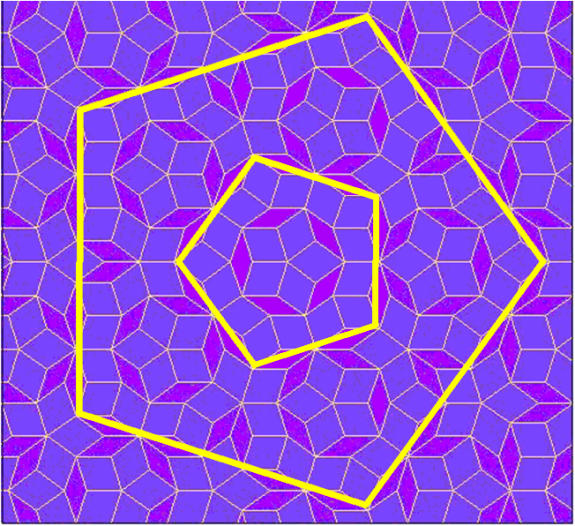
\includegraphics[width=60mm]{./figure/quasicrystalline_structure1.jpg}
  \caption{準結晶の結晶構造}
  \label{quasicrystalline_structure1}
\end{figure}

\section{研究目的}
本研究では、Au-Al-Tb系1/1近似結晶の磁気基底状態の解明を目的としている。図\ref{purpose_of_research}に示すように、通常の結晶は周期的な構造を持つため、スピンが揃いやすく磁気秩序を形成しやすい。一方、アモルファスのようなランダムな構造ではスピン秩序は見られないことが知られている。近年、多くの準結晶が発見され、これらの準結晶の局所構造をもつ近似結晶を用いた研究が進展し、準結晶に関する理解が深まってきた。特に、ランタノイド元素を含む準結晶や近似結晶では、長距離磁気秩序を示す例が報告されているが、準周期構造を持つ準結晶のスピン構造については、いまだに明らかになっていない。そこで本研究では、Au-Al-Tb系1/1近似結晶に対してAC磁化率測定およびAl-NMR測定を行い、マクロ測定とミクロ測定両方の観点から準結晶・近似結晶における磁気基底状態を明らかにすることを目指す。

\begin{figure}[htbp]
  \centering
  \vspace{10mm}
  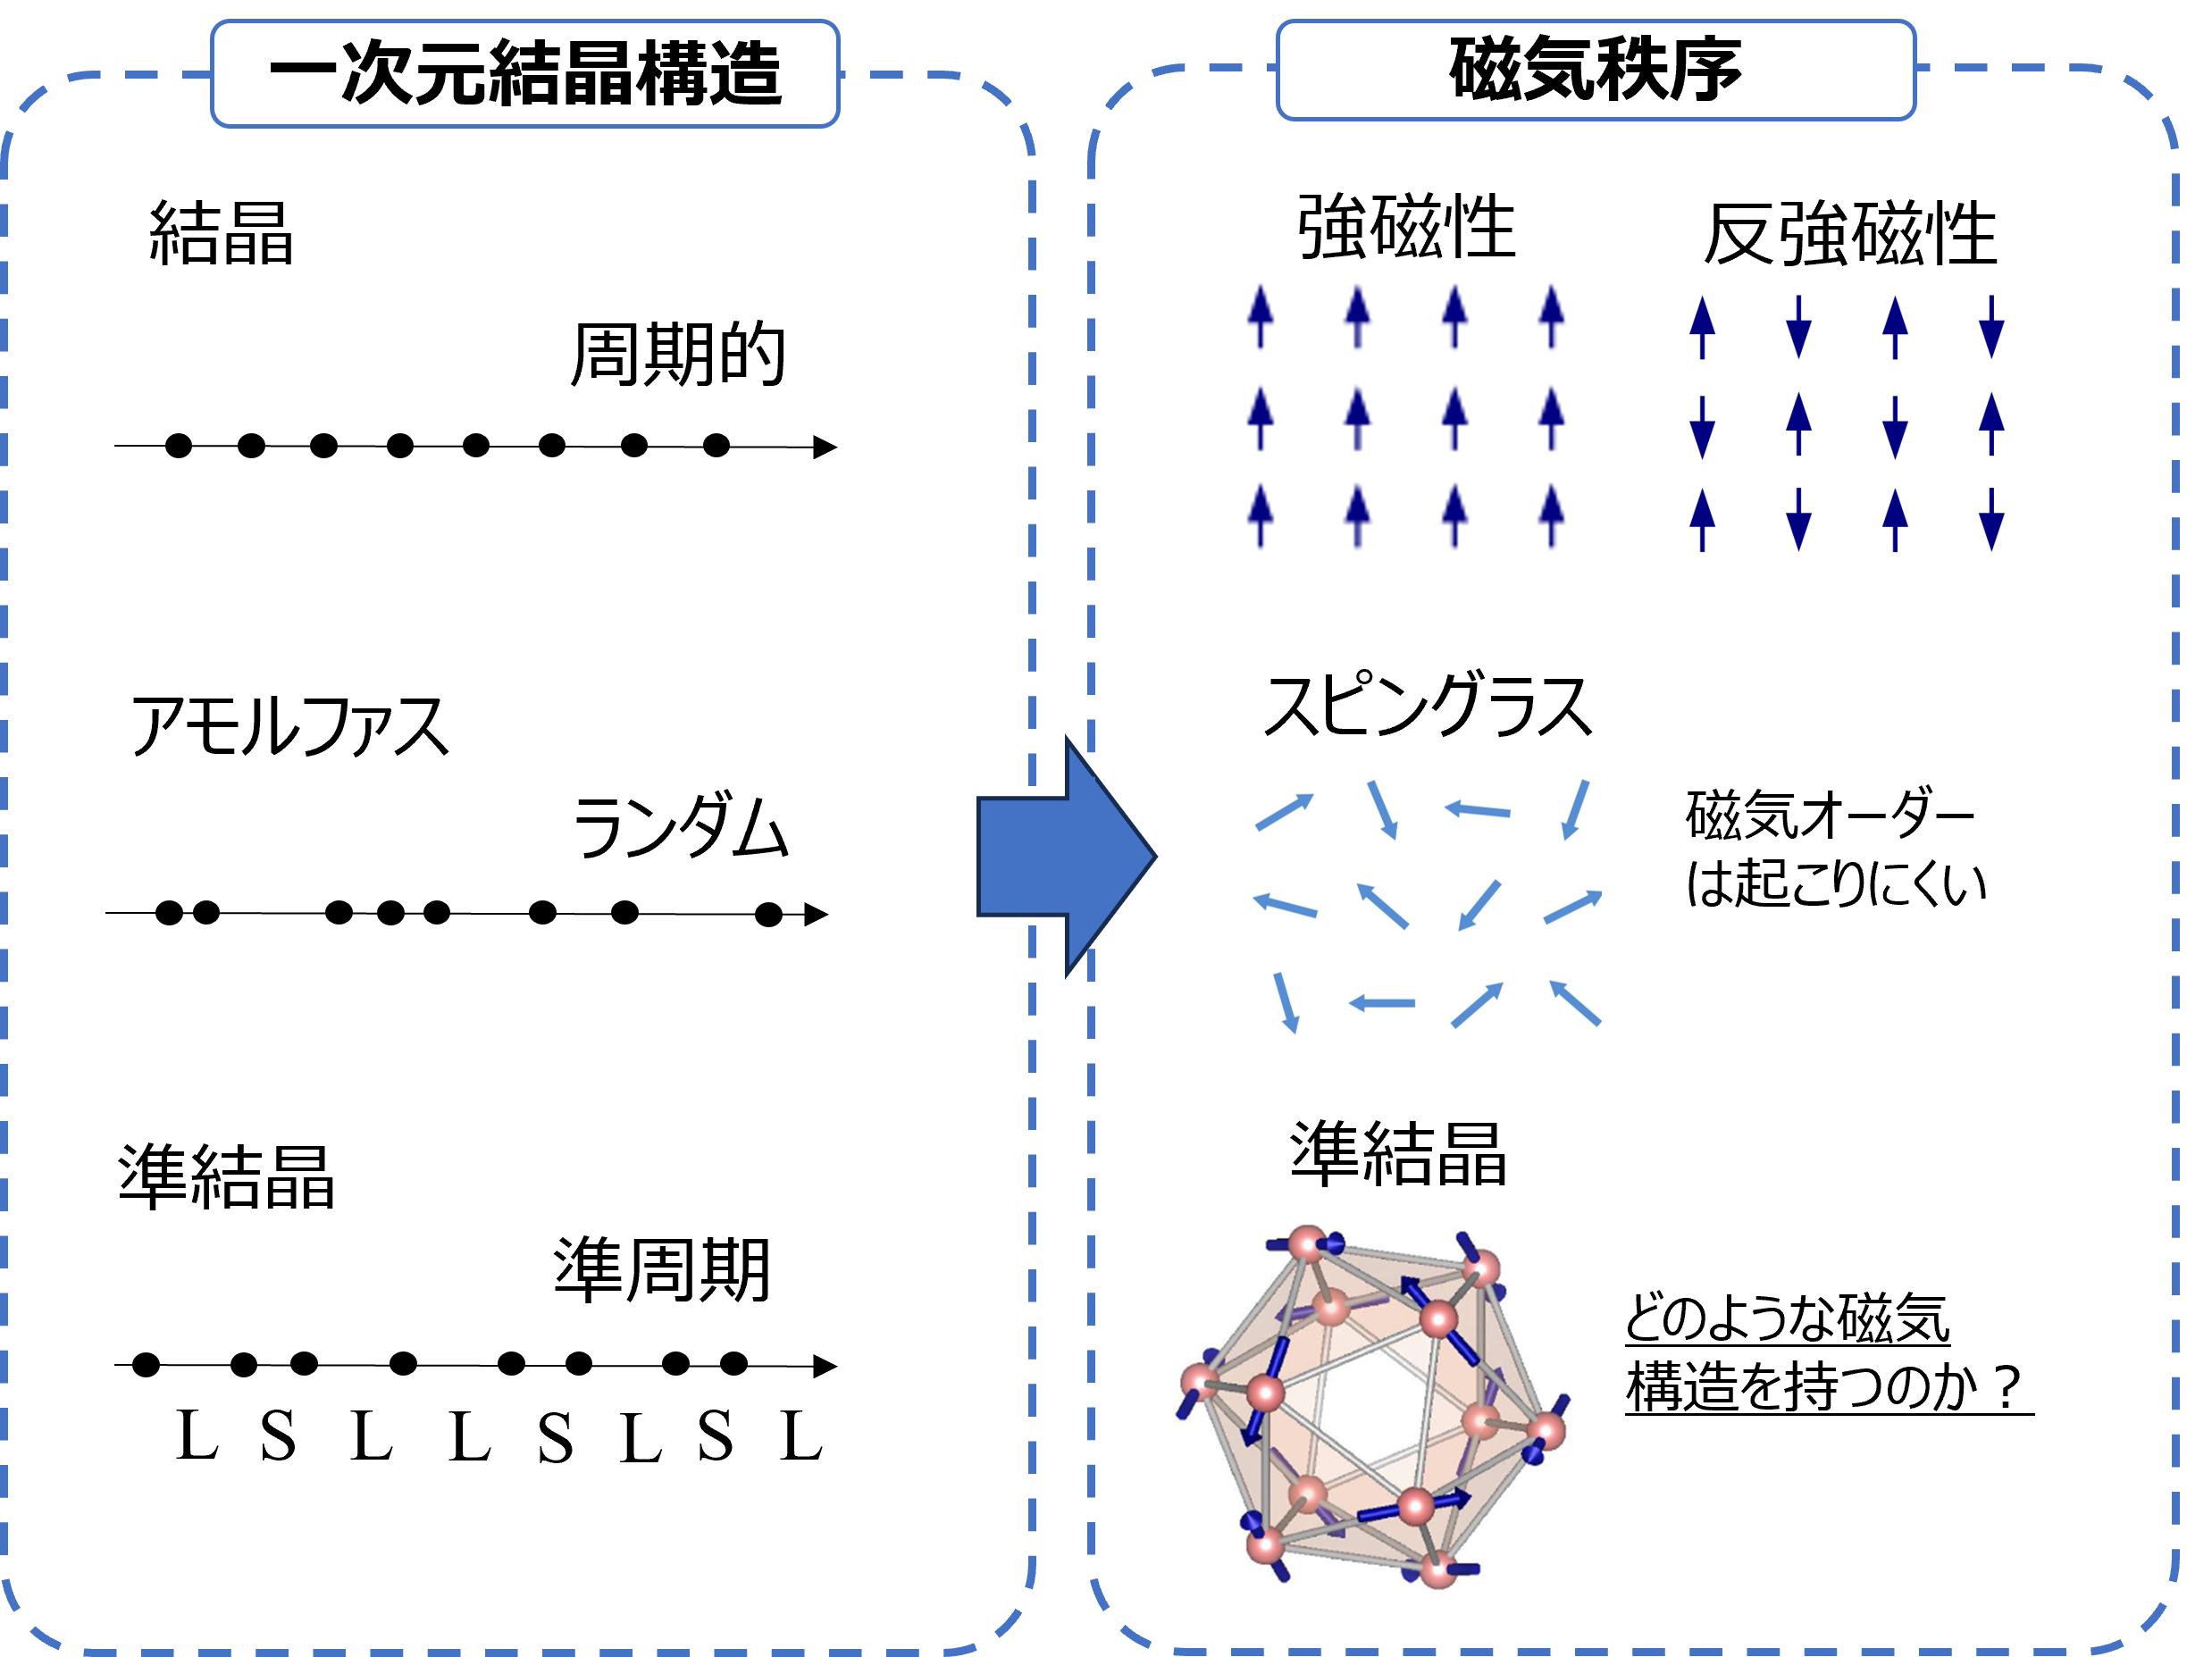
\includegraphics[width=140mm]{./figure/purpose_of_research.png}
  \caption{研究目標}
  \label{purpose_of_research}
\end{figure}
\chapter{準結晶}
\section{準結晶の定義}\label{準結晶の定義}
準結晶は、1章でも紹介した通り、通常の結晶が持つ原子配列秩序とは異なる新しいタイプの原子配列秩序を持った個体物質である。一般に固体の原子配列秩序、とくに長距離秩序、すなわち最近接原子間距離に比べて十分長い距離にわたって存在する秩序は、
X線や電子線の回折スペクトルに端的に現れる。ここで、個体に入射した平面波が固体中の原子により散乱される場合を考える。電子密度を与える関数を$\rho({\bm r})$とし、散乱ベクトルを$\bm S$すると散乱波の足し合わせ$F(\bm S)$は
\begin{equation}
  F(\bm S)=\int{\rho(\bm r)} \exp (-2\pi i \bm S\cdot\bm r)d\bm r
\end{equation}
で表される。ここで、$\bm r$が張る空間が実空間なのに対して、$\bm S$が張る空間を逆空間という。\\
さらに散乱強度$I(\bm S)$は、
\begin{equation}
  I(\bm S) =  |F(\bm S)|^2
\end{equation}
で与えられる。$I(\bm S)$の性質は秩序性の観点から個体を分類する。\par
もし、個体がアモルファス(非結晶)なら、散乱強度$I(\bm S)$は連続的な関数となり、これは長距離秩序を持たないことを意味する。一方、個体が「広義の結晶」である場合$I(\bm S)$は、$\delta$関数のセットとなり
\begin{equation}
  I(\bm S) =  \sum_{i}{|A_i|^2\delta(\bm S- \bm G_i)}
\end{equation}
の回折スペクトルとなる。ここで、$\delta$の位置の集合${\bm G_i}$は逆格子である。
逆格子{$\bm G_i$}のあらゆる要素がある有限個のベクトルの組$\bm a_i^*(i=1,2,\cdots,N)$の整数線形結合で表せるとき、$a_i^*$を逆格子基本ベクトルという。最小の逆格子基本ベクトルの数を$N$とすると、並進対称性をもつ「狭義の結晶」では、その数$N$は空間の次元数$d$と一致する。一方、$N>d$となる「非周期結晶」の場合、空間次元の周期性を持たない、もし$N$が空間次元数より大きければそれは「非周期結晶」とよばれる。\par
また、2次元または3次元の「狭義の結晶」に許される回転対称性は2,3,4,6回に限られる。すなわち、それら以外の回転対称性は2次元、3次元の周期性と両立しない。しかし、「非周期結晶」ではその限りではなく、なかでも$I(\bm S)$が「狭義の結晶」に存在しない回転対称性、すなわち2,3,4,6回以外の回転対称性をもつ場合、そのような構造を「準結晶」とよび、そうでないものを「非整合結晶」と呼ぶ。
\section{準結晶格子}
\ref{準結晶の定義}節の準結晶の定義を満たす構造のなかで、少数個の単位胞の充填構造からなるものを一般に「準結晶格子」とよぶ。準結晶格子は、実際の準結晶物質の原子配列構造記述する上で重要な役割を果たすものである。本節では、典型的な準結晶格子である2次元ペンローズ格子、3次元ペンローズ格子について説明する。しかし、その前に、厳密には「準結晶格子」とはいえないが、2次元、3次元のペンローズ格子と密接に関系する1次元フィボナッチ格子について説明する。1次元フィボナッチ格子は次元が低いので、準結晶格子やそのフーリエ変換の一般的な記述法、またそれらに関連する重要な概念を記述するのに適している。
\begin{figure}[htbp]
  \centering
  \vspace{10mm}
  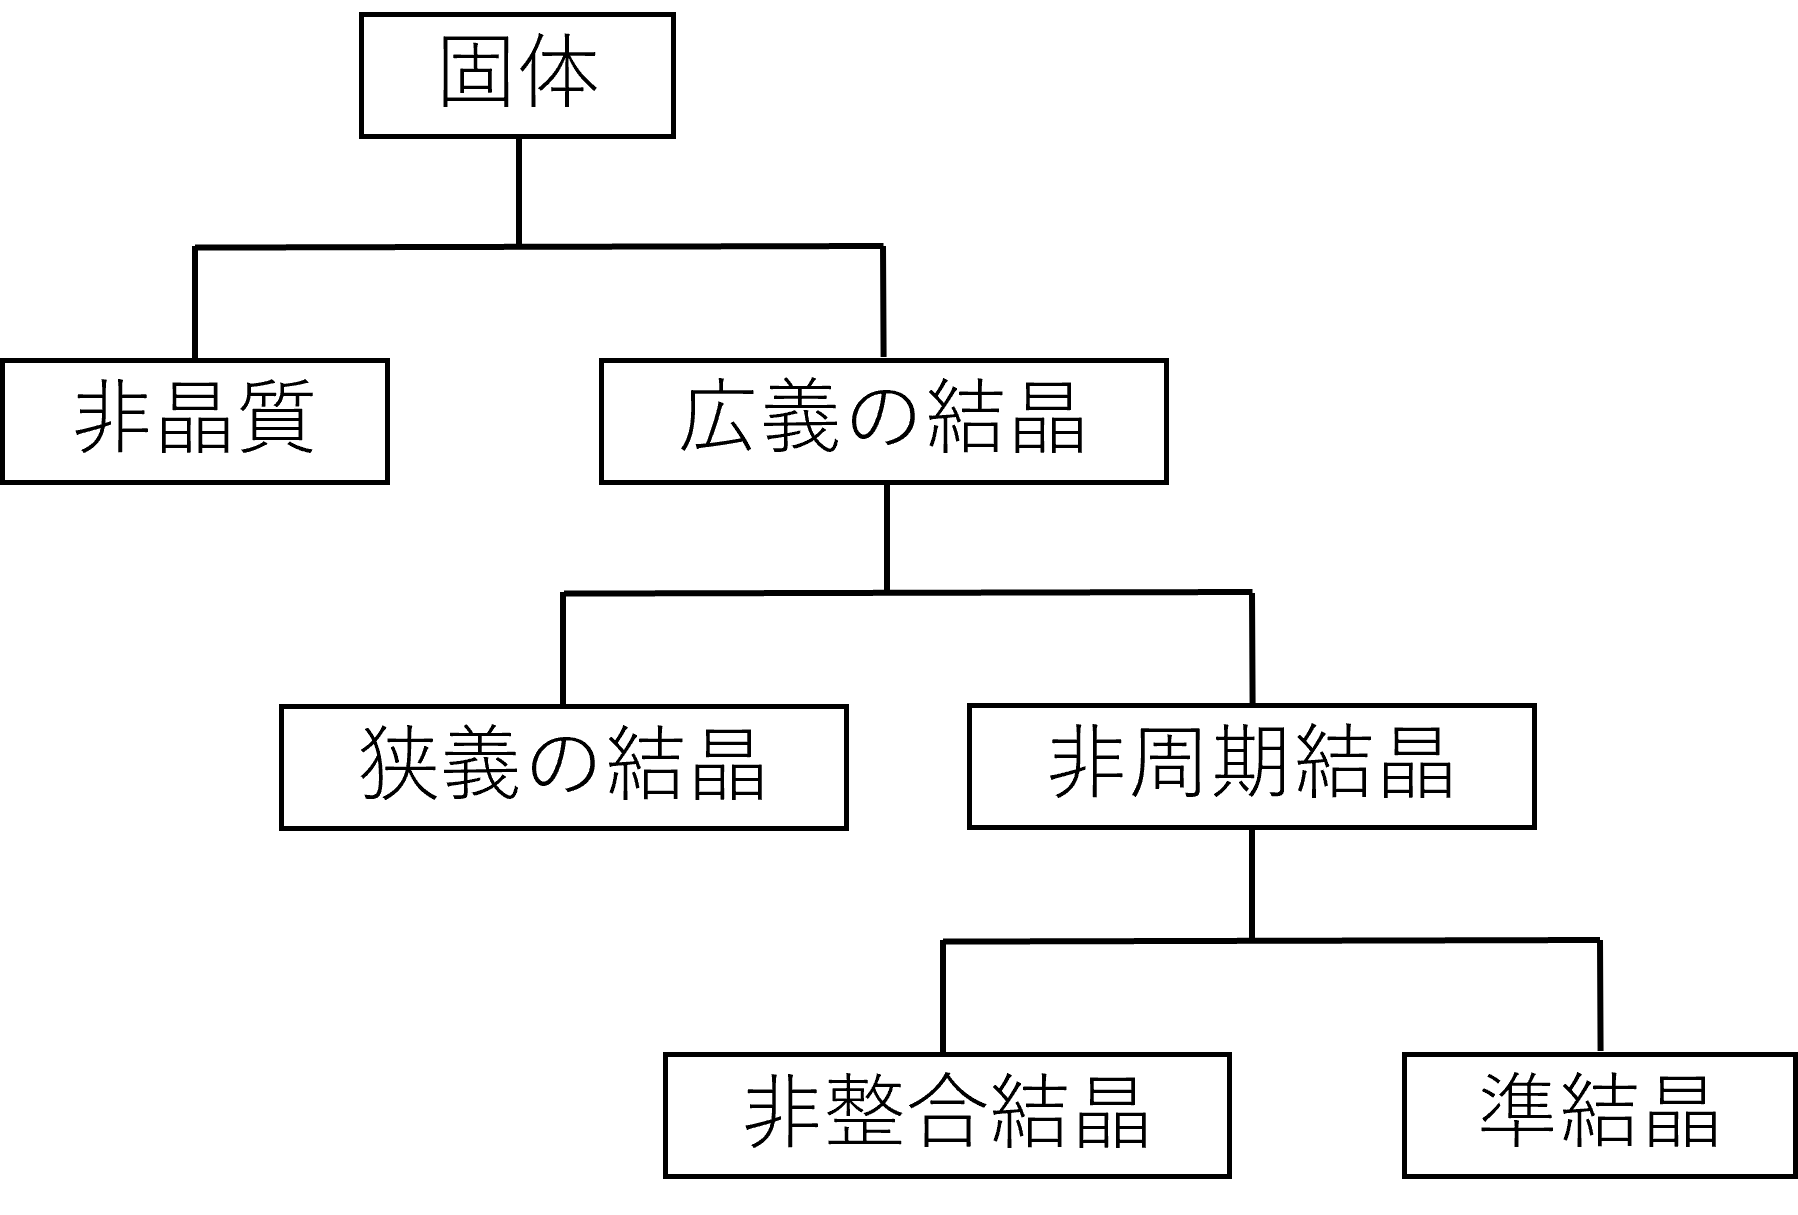
\includegraphics[width=120mm]{./figure/quasicrystalline_define.png}
  \caption{準結晶の定義}
  \label{quasicrystalline_define}
\end{figure}
\subsection{1次元フィボナッチ格子}
1次元においては\ref{準結晶の定義}でも説明した準結晶の定義である1,2,3,4,6以外の回転対称性を持っているという構造が存在しないので、厳密には1次元準結晶格子というものは存在しない。しかし、少数個の単位胞からなる1次元準周期構造は存在するので、ここではこれらを「1次元準周期格子」と呼ぶことにする。1次元準周期格子のような構造は、2次元の典型的な準結晶格子である2次元の典型的な準結晶格子である2次元ペンローズ格子や、後述する3次元の典型的な準結晶格子である3次元ペンローズ格子の中に見出すことができるので、それらの構造を理解する上で重要である。特に黄金比$\tau=(1+\sqrt5)/2$の基本長さの比をもつ1次元準周期格子「フィボナッチ格子」の構造は2次元、3次元のペンローズ格子の構造と密接に関係している。ここではこのフィボナッチ格子について述べる。\par
フィボナッチ格子は長さの比が$\tau$の2種類の間隔LとS(longとshotの意味)がいわゆるフィボナッチ配列をした構造を持つ。フィボナッチ配列は次のように定義される。まず、Lを第1世代としてこれを$\tau:1$に内分すると第2世代の配列LSが得られる。これのLをさらに$\tau:1$に内分すると第3世代のLSLが得られる。ここで第2世代のSの長さを1とすると第2世代のLは$\tau$であり、これを$\tau:1$に内分すると$\tau\cdot\tau/(\tau+1)$の2つの長さが生ずる。$\tau^2=\tau+1$なのでこれらは1と$1/\tau$になり、第2世代のSはそのまま第3世代のLになる。このような変換を無限に繰り返すことにより、図\ref{fibonacci_lattice}に示すような、LとSからなるフィボナッチ格子が得られる。この作り方から、フィボナッチ格子が$\tau$倍のスケール変換に関する自己相似性をもつことがわかる。
\begin{figure}[htbp]
  \centering
  \vspace{10mm}
  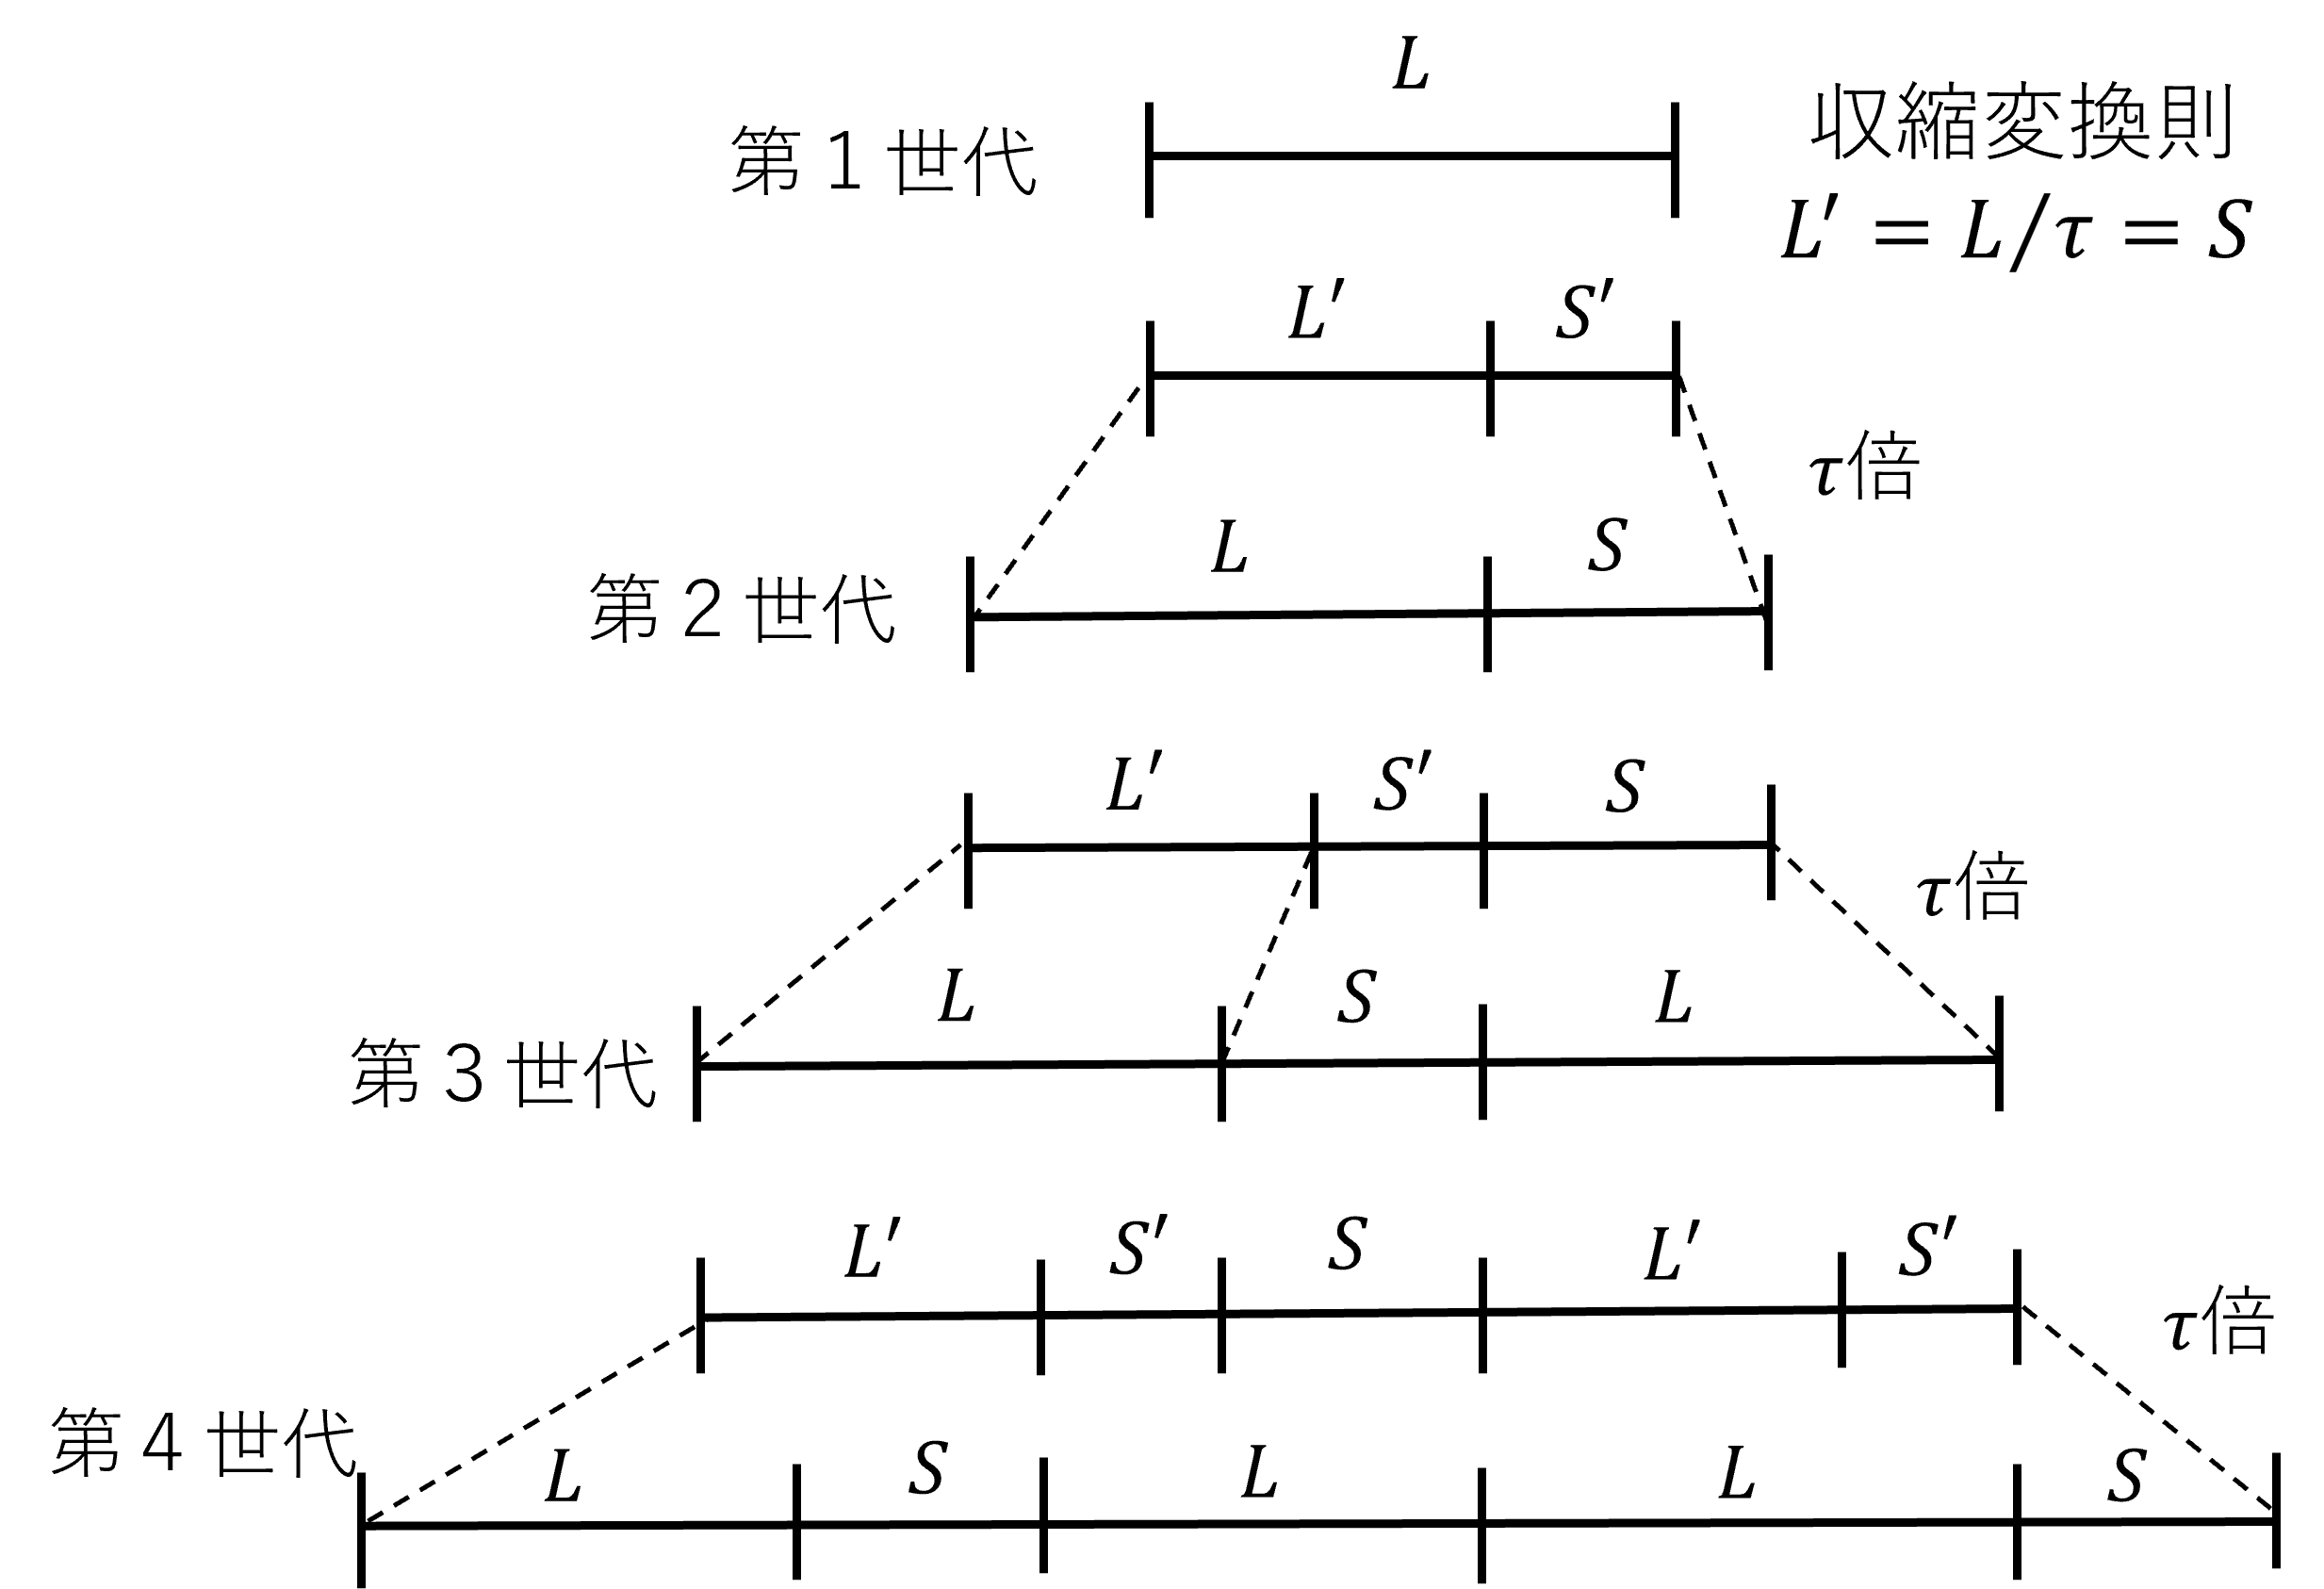
\includegraphics[width=120mm]{./figure/fibonacci_lattice.png}
  \caption{フィボナッチ格子}
  \label{fibonacci_lattice}
\end{figure}
フィボナッチ配列では第$n$世代$(n\ge3)$は、第$(n-1)$世代の後ろに第$(n-2)$世代をくっつけたものになっている。第$n$世代のLとSの総数を$F_n$とおくと、このような関係から
\begin{equation}
  F_n = F_{n-1}+F_{n-2}\quad (n\ge3)
\end{equation}
が成り立つ。$F_1=1,F_2=2$としてこの漸化式で定義される数列$1,2,3,5,8,13,\cdots$はフィボナッチ数列よばれる。




\subsection{2次元ペンローズ格子}
2次元準結晶格子には5,8,10,12回の回転対称性をもつものが存在する。なかでも、回折パターンに10回回転対称性を持つ準結晶格子は2次元ペンローズ格子と呼ばれる代表的な準結晶格子である。この格子は、2種類の菱形(厚い菱形と薄い菱形)を特定のタイル張りルールに従って構成され、各タイルは角度が72度と36度を持ち、黄金比$\tau=(1+\sqrt{5})/2$に関連にした寸法を有する。さらにペンローズ格子は自己相似性を特徴とし、拡大や縮小を行っても同様のパターンが現れる。これはスケール不変性と呼ばれ、準結晶の特性の一つである。
また、2次元ペンローズ格子とその回折像は、フーリエ変換で結ばれており、5回回転対称性をもつ2次元ペンローズ格子をフーリエ変換すると10回回転対称性をもつ回折像になり、逆に回折像からフーリエ逆変換をすることにより、実空間における2次元ペンローズ格子が得られる。
\begin{figure}[htbp]
  \centering
  \vspace{3mm}
  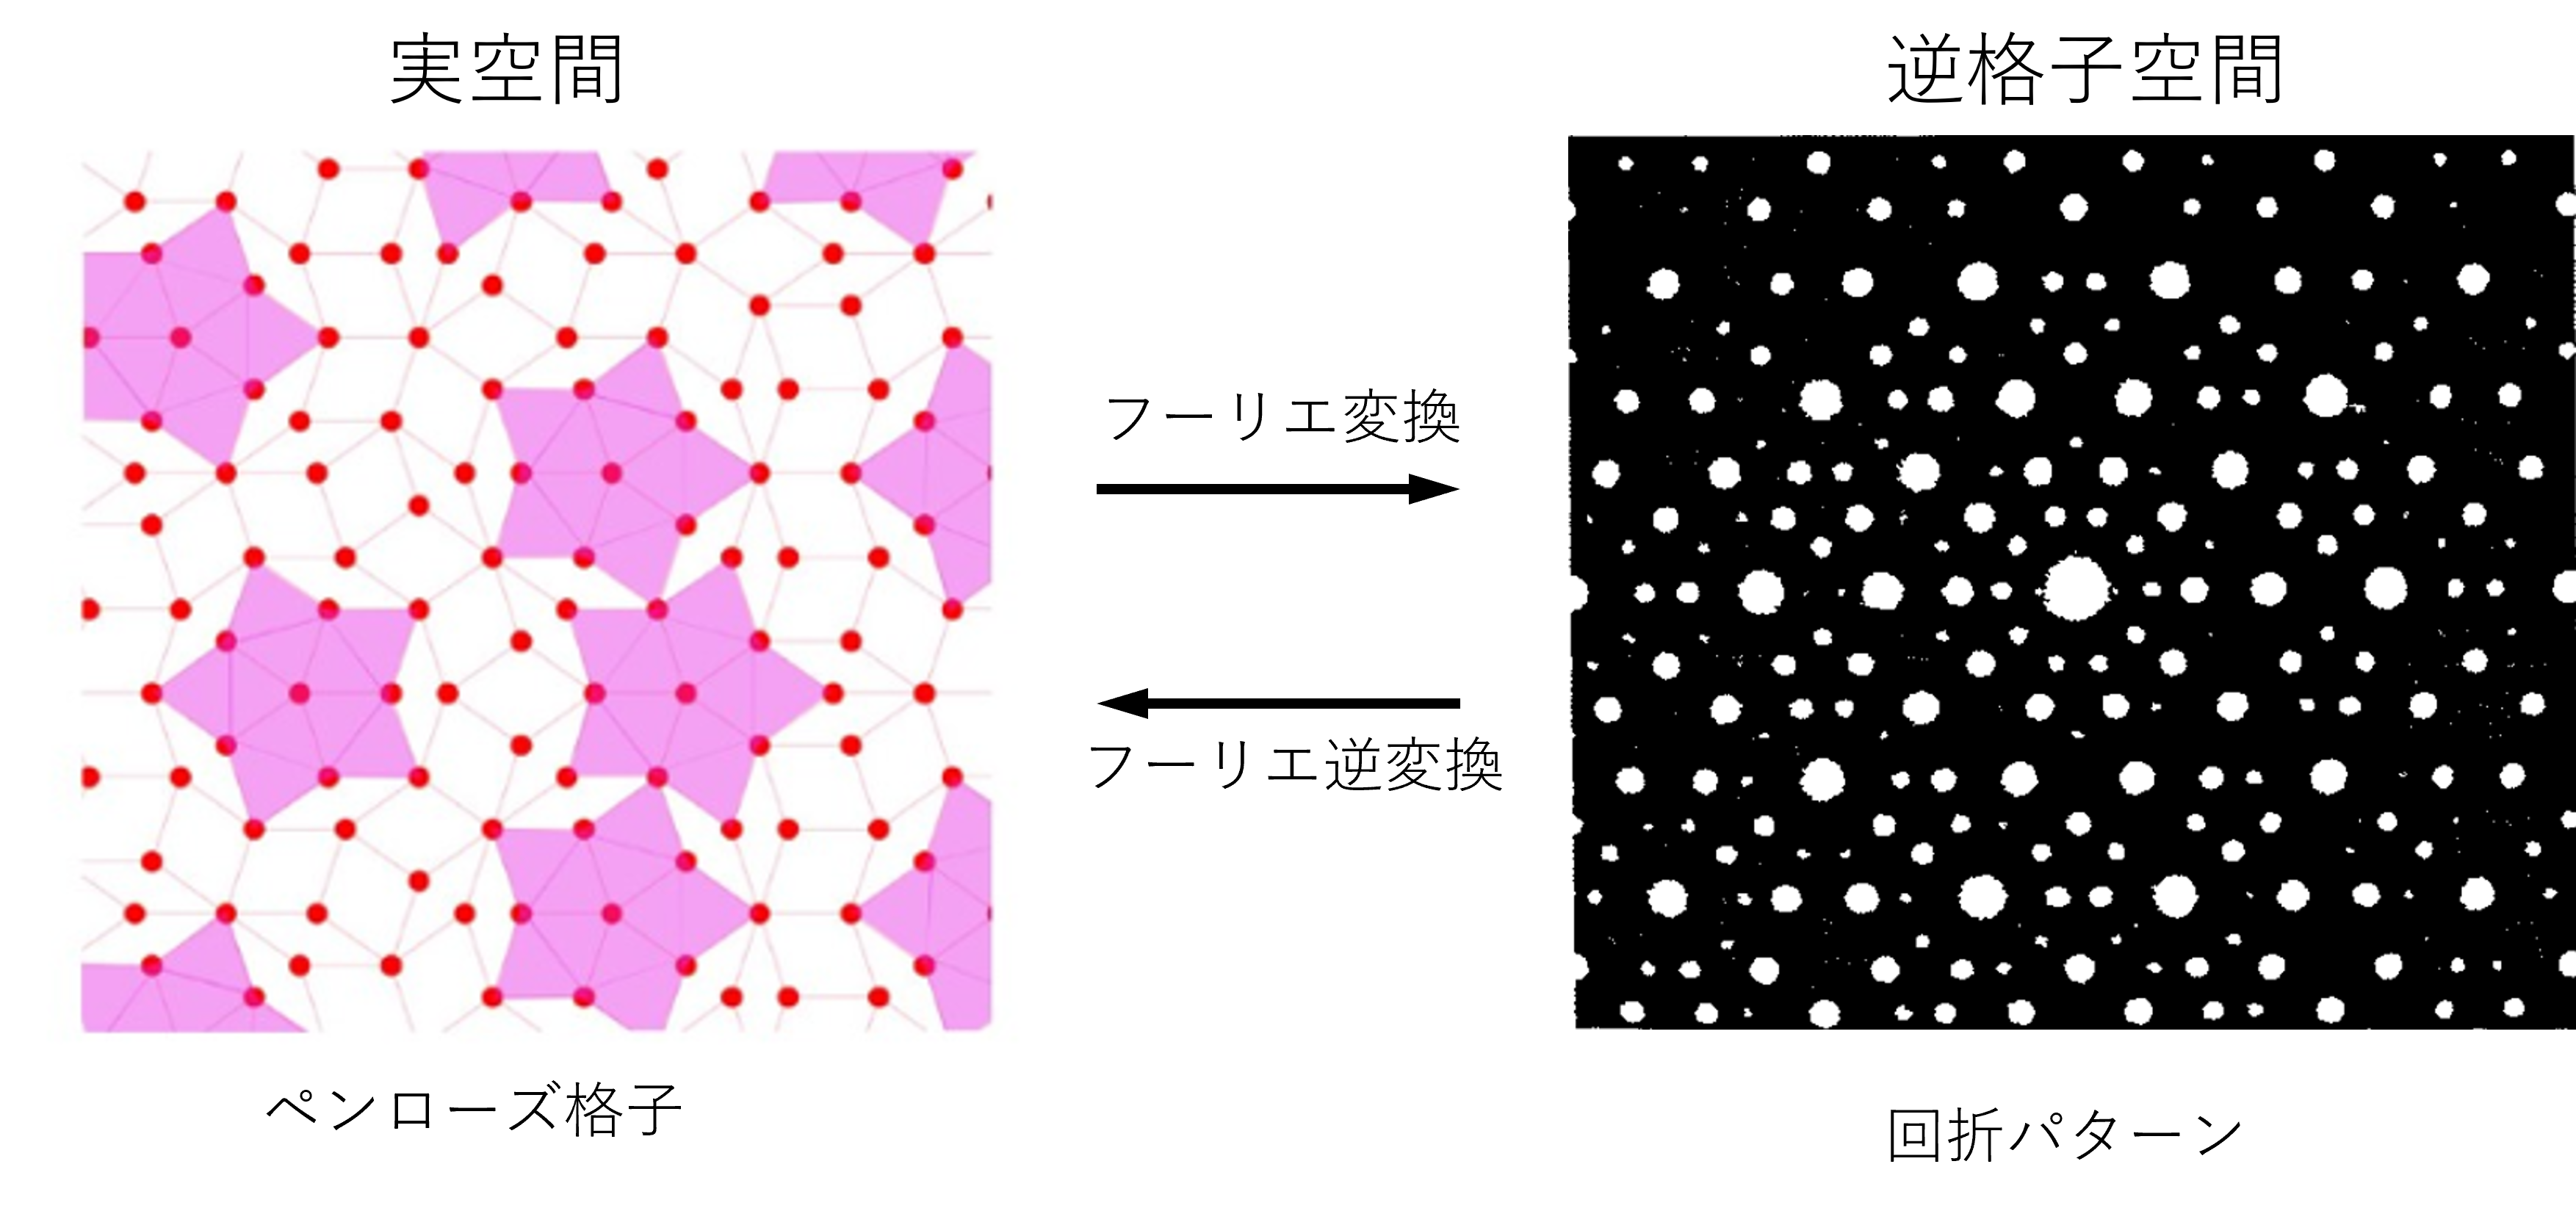
\includegraphics[width=150mm]{./figure/penrose_tile.png}
  \caption{2次元ペンローズ格子と回折像}
  \label{penrose_tile}
\end{figure}

\subsection{3次元ペンローズ格子}
3次元ペンローズ格子は、5次元空間で正20面体対称性を持つ周期的な格子を3次元空間に射影することで得られる特殊な構造である。高次元の周期的な格子から適切な部分を選び出し、それを低次元の物理空間に射影することで、非周期的でありながら秩序だったパターンを形成することができる。この5次元から3次元への射影過程では、正20面体の対称性は維持され、ペンローズ格子にもこの特異な対称性が反映される。結果として、通常の周期的な格子では実現できない5回対称性などの特徴が現れ、ペンローズ格子の非周期性と長距離秩序を説明することができる。

\subsection{高次元投影法}\label{高次元投影法}
高次元の周期的な格子構造を利用して、低次元での準周期的な構造を生成する方法を高次元投影法と呼ぶ。これにより、高次元空間でのシンプルな構造を低次元に投影することで複雑な準周期構造を理解することに役立つ。ここでは、1次元準周期格子を例にあげ、高次元投影法について説明する。
1次元準周期構造の回折関数$F(\bm S)$は、長さの比が黄金比$\tau$になる2つの基本逆格子ベクトル$\bm a_1^*,\bm a_2^*$を用いて表すことができ
\begin{equation}
  F(\bm S) = \sum_{n_1}\sum_{n_2}{A_{n_1,n_2}\delta(S-(n_1\bm a_1^*+n_2\bm a_2^*))}
  \label{F_S}
\end{equation}
となる。これをフーリエ逆変換して逆空間の関数$F(\bm S)$から実空間の関数$\rho(\bm r)$に直すと
\begin{equation}
  \rho(\bm r)=\sum_{n_1}\sum_{n_2}{A_{n_1,n_2}\exp[2\pi i(n_1\bm a_1^*+n_2\bm a_2^*)\cdot\bm r]}
  \label{rho_r}
\end{equation}
となる。このような1次元準周期構造は、ある2次元周期関数の1次元断面として記述できることが以下のようにしてわかる。まず式(\ref{rho_r})に対して関数$\rho^h(t_1,t_2)$($h$は高次元関数または高次元ベクトルを表す添え字)を次式で定義する。
\begin{equation}
  \rho^h(t_1,t_2)=\sum_{n_1}\sum_{n_2}{A_{n_1,n_2}\exp[2\pi i(n_1t_1+n_2t_2)]}
  \label{rho_t}
\end{equation}
これは、$t_1,t_2$に関して周期1の周期関数になっている。式(\ref{rho_r}),式(\ref{rho_t})より
\begin{equation}
  \rho(\bm r)=\rho^h(t_1,t_2)
  \label{rho_r_t}
\end{equation}
ただし,
\begin{equation}
  \left\{
    \begin{aligned}
      t_1 = \bm a_1^*\cdot\bm r \\
      t_2 = \bm a_2^*\cdot\bm r
    \end{aligned}
 \right.
\end{equation}
ここで$\bm a_1^*,\bm a_2^*$の比から
\begin{equation}
  t_2=\tau t_1
  \label{t_t}
\end{equation}
である。このことから、1次元準周期関数$\rho(\bm r)$が2次元周期関数$\rho^h(t_1,t_2)$の式\ref{t_t}であらわされる直線上の値として得られることがわかる。\par
図\ref{High_dimensional_projection}にこのような形で記述した1次元準周期構造の例を示す。基本周期ベクトル$\bm d_1,\bm d_2$を図のように$|\bm d_1|=|\bm d_2|,\bm d_1\perp \bm d_2$をみたすようにとる。ここで、2次元空間内で関数$\rho(\bm r)$が得られる1次元部分空間を$E_\parallel$,それと直交する補空間を$E_\perp$と名付ける。2次元周期関数としては各格子点に$E_\perp$方向に伸びた線分がくっついたものを考えており、この関数は線分上でのみ$\delta$関数的に値をもち、他では値が0である。よって、$E_\parallel$上の1次元密度関数$\rho(\bm r)$は、2次元周期関数との交点で値を持つ$\delta$関数のセットからなり、さらに$\delta$関数の長さには適当な下限と上限があるので、実際の原子配列の1次元的なモデルになりうるものである。$E_\perp$方向にのびた線分が$E_\parallel$と交差する点が$E_\parallel$上で原子位置に対応し、この線分は高次元空間(hyperspace)の原子という意味で「超原子」(hyperatom)とよばれる。
\begin{figure}[htbp]
  \centering
  \vspace{3mm}
  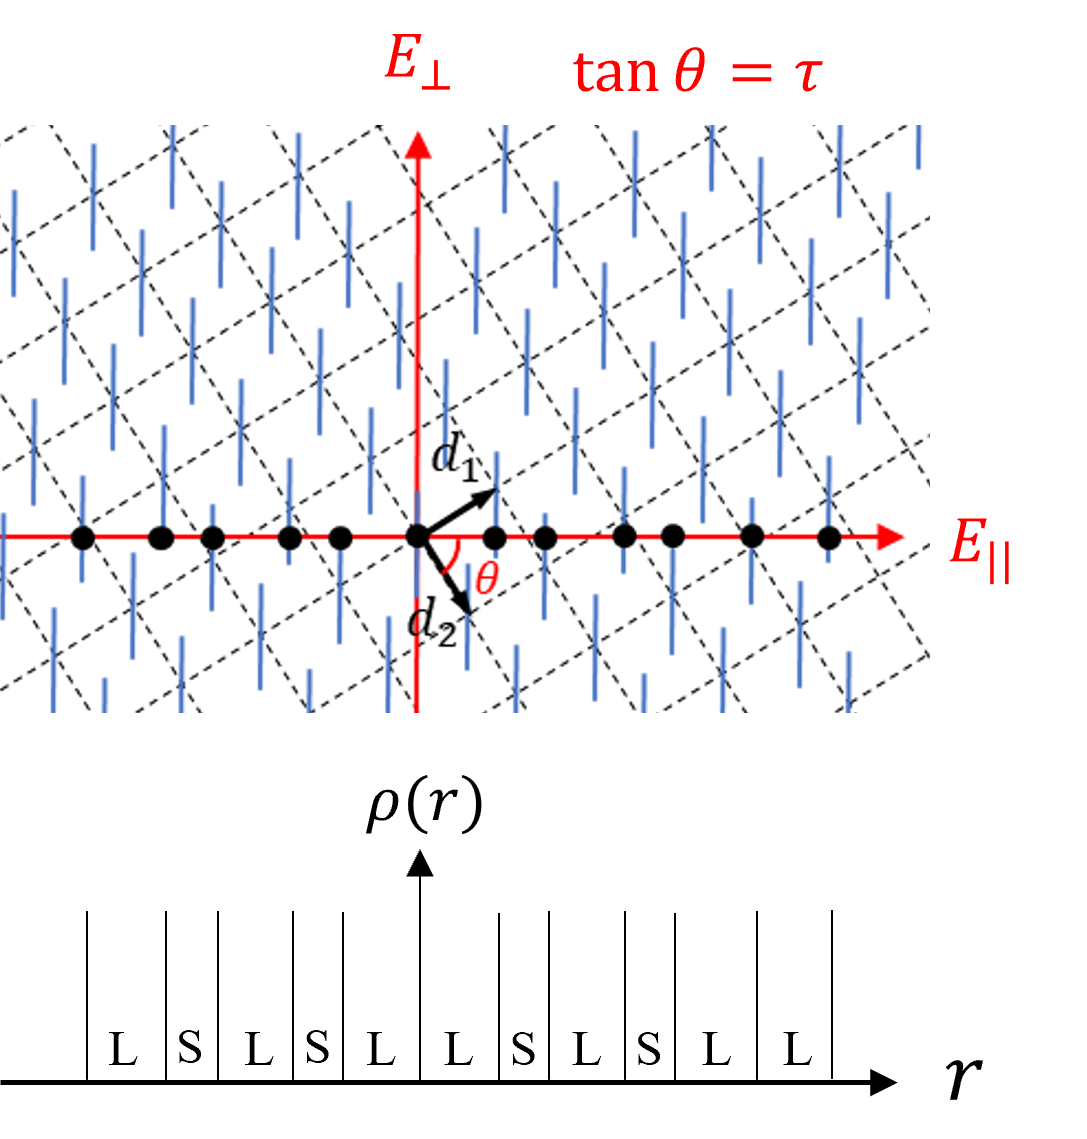
\includegraphics[width=100mm]{./figure/High_dimensional_projection.png}
  \caption{高次元投影法}
  \label{High_dimensional_projection}
\end{figure}
\section{近似結晶}
近似結晶は、準結晶と密接な関係を持ちながら、周期的な結晶構造を有する物質である。準結晶は、従来の結晶学の枠組みでは禁じられていた対称性、例えば五回回転対称性や十回回転対称性を示す非周期的な構造を持つことで知られているが、近似結晶はこれらの準結晶と類似した局所的な原子配置や対称性を持ちつつ、全体としては周期的な構造を維持している。この周期性は、大きな単位胞内に多数の原子が配置され、その単位胞が空間内で周期的に繰り返されることにより実現している。\par
近似結晶の形成には、フェイゾン歪と呼ばれる特殊な歪みが関与している。フェイゾン歪は、準結晶における追加の自由度であるフェイゾン自由度に起因し、この歪みを導入することで非周期的な準結晶構造が周期的な結晶構造に変換される。一次元の準結晶モデルであるフィボナッチ格子において、フェイゾン歪を導入すると、\ref{高次元投影法}節の高次投影法において逆格子ベクトルの比が有理数(つまり、$\tan \theta$が有理数)となり、投影された格子の関数$\rho(r)$は周期的になる。この有理数の比はフィボナッチ数列に関連し、例えば逆格子ベクトルの比が $1/1, 2/1, 3/2,\dots,F_{n+1}/F_n$ となると、1周期内の配列もLS,LSL,LSLLS,…のように増えていき、$n$の値が多きくなるにつれて準結晶構造に近くなる。ここで、$1/1$ の場合は 1/1 近似結晶、$2/1$ の場合は 2/1 近似結晶と呼ばれる。\par
また、近似結晶の研究は、準結晶の複雑な構造や物理的性質の解明において重要な役割を果たす。準結晶はその非周期的な構造のために直接的な解析が難しいが、周期構造を持つ近似結晶を解析することで、準結晶の構造に関する間接的な情報が得られる。特に、近似結晶の原子配列や対称性、電子構造などを調べることで、準結晶における物理的特性の予測や理解が進むと考える。

\begin{figure}[htbp]
  \centering
  \vspace{10mm}
  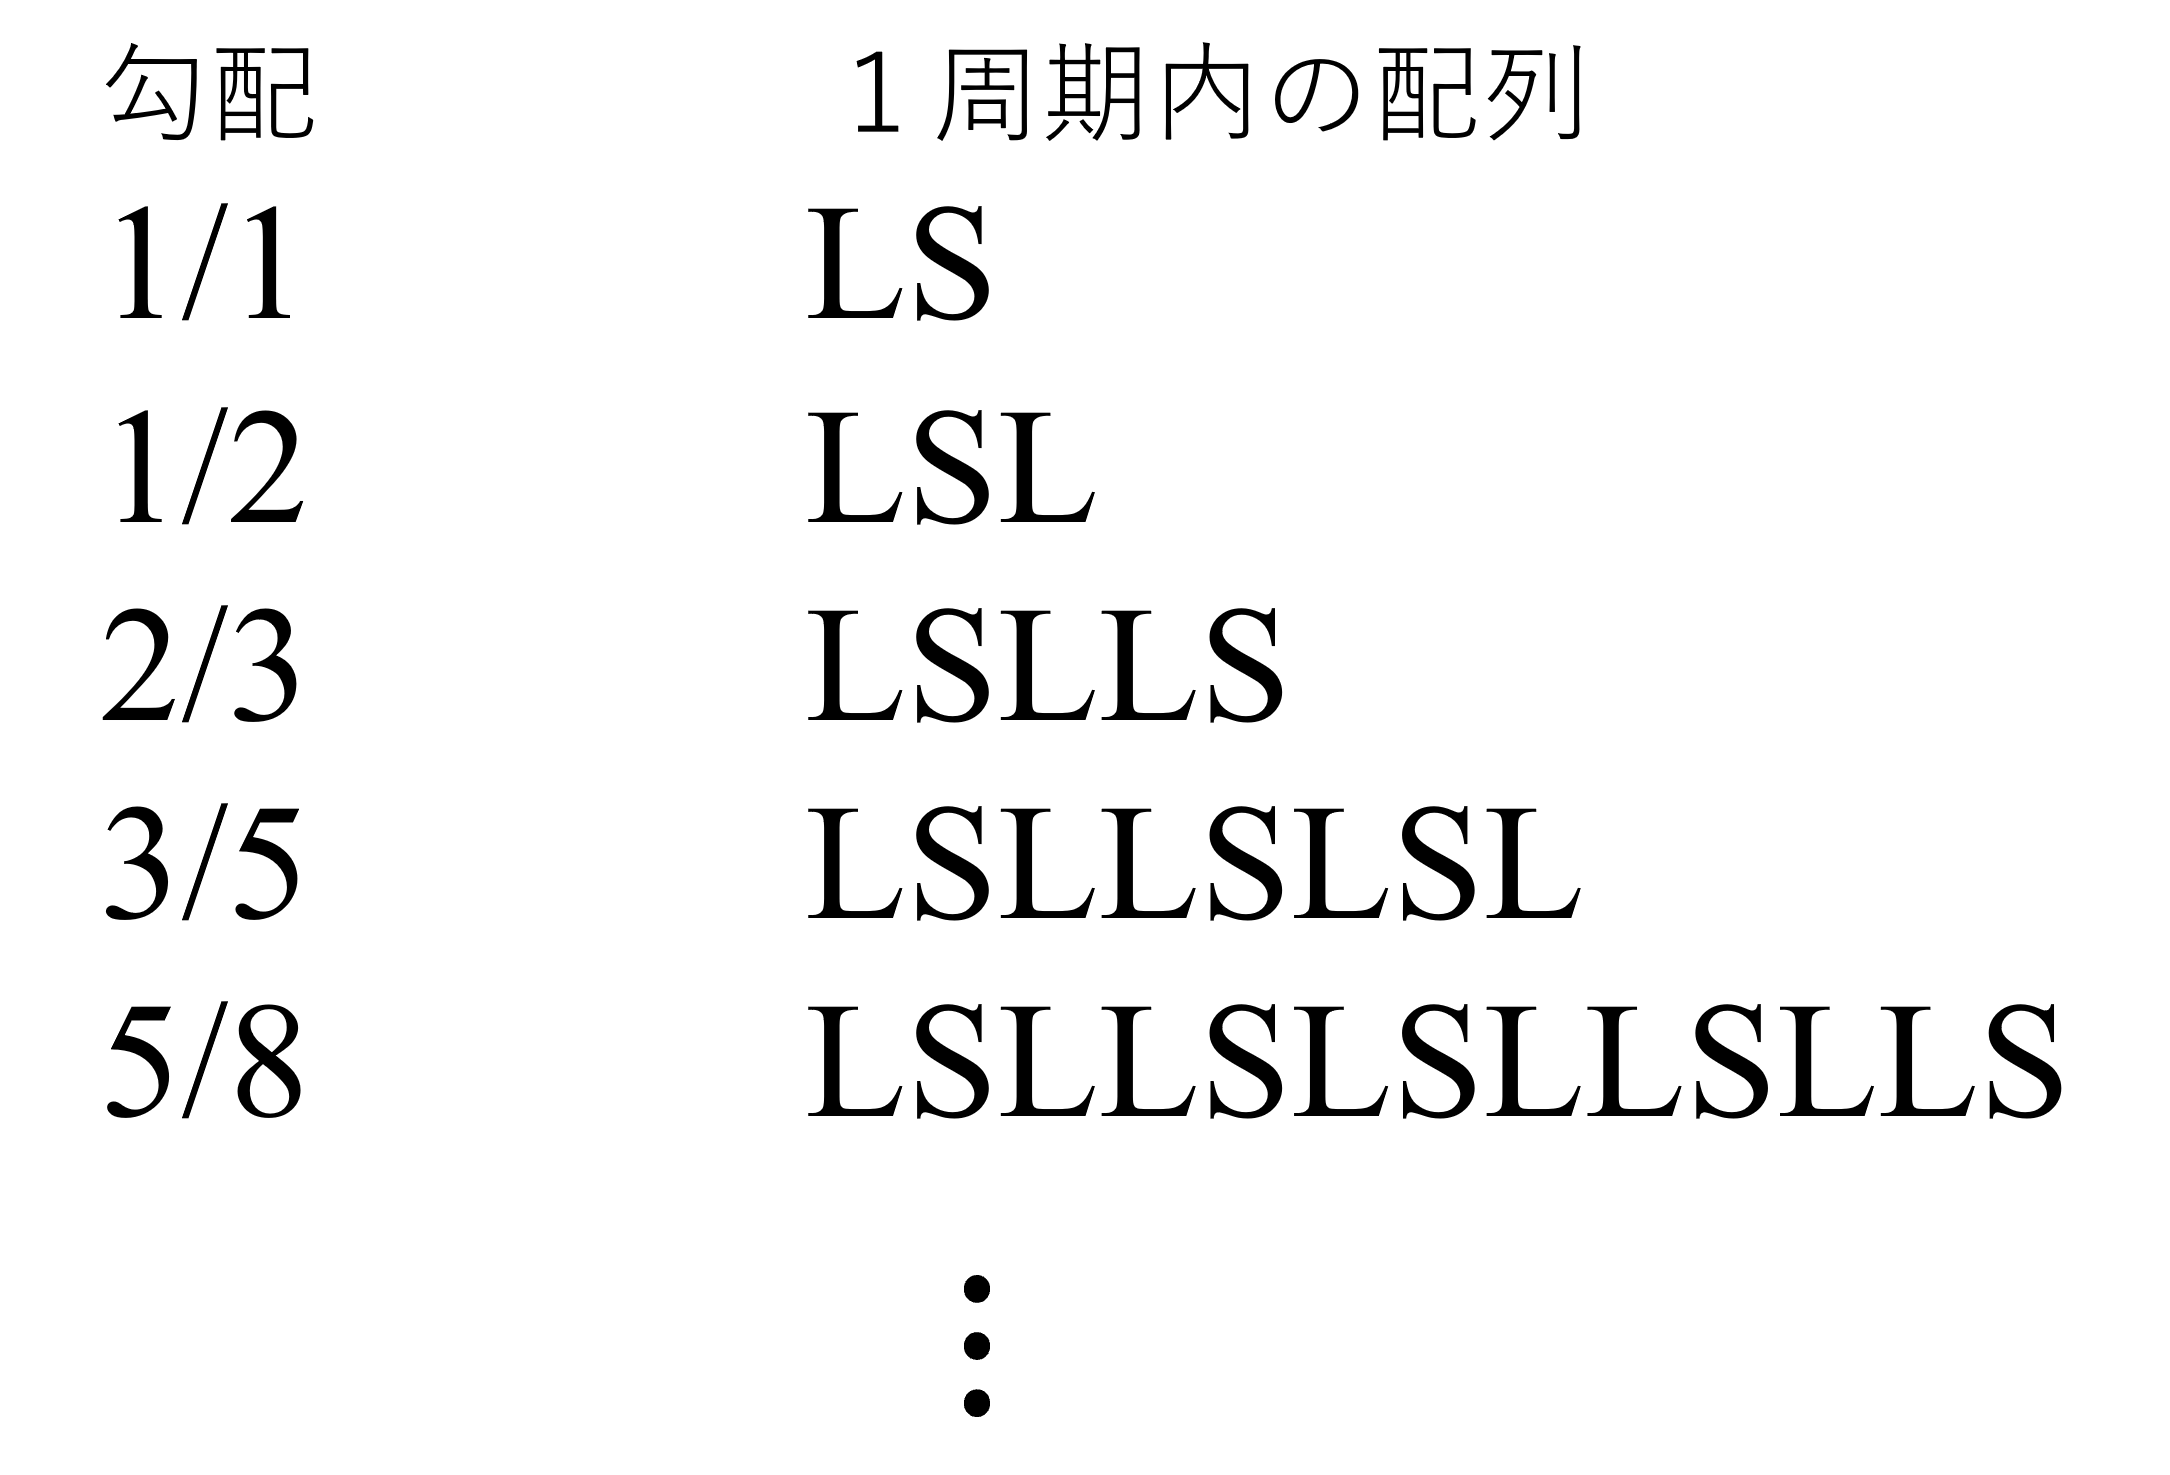
\includegraphics[width=100mm]{./figure/LS.png}
  \caption{逆格子ベクトルの比と1周期内の配列}
  \label{LS}
\end{figure}
\chapter{先行研究}
\section{Tsai型近似結晶の磁性}
2021年東京理科大学の鈴木氏らは、Tsai型準結晶近似体の磁性に関する包括的な調査を行い、特に1/1および2/1近似体の磁気的性質について詳述している。
本研究の主な焦点は、希土類元素(R)を含むTsai型1/1近似体において、電子数(e/a比)が磁気秩序に与える影響である。e/a比は準結晶やその近似体の磁気挙動を制御する重要なパラメータであり、特に磁化のCurie-Weiss温度($\theta_p$)や磁気秩序がe/a比に応じて系統的に変化することが示された。\par
Tsai型近似体の磁化率測定では、異なるe/a比に対応して強磁性(FM)、反強磁性(AF)、およびスピングラス的な状態が観察された。
特に、反強磁性状態では磁化率が低温で尖ったピークを示し、反強磁性転移温度($T_N$)が特定された。
スピンフロップ現象が低磁場で見られたことから、異なる磁気秩序が存在することが示唆された。
さらに、e/a比が1.54から2.16の範囲で、AF、FM、スピングラスの各領域が交互に出現することが観察され、特に反強磁性領域がTb系で広がっていることが示唆されている。
ピン系における異方性が磁気秩序の形成に重要な役割を果たしていることも示唆され、1/1近似体の磁気相図が2/1近似体にも適用できる可能性が明らかになった。
磁化率測定の結果からも、Tsai型準結晶近似体の磁気相が電子数に依存して変化することが確認され、今後の準結晶やその近似体における未発見の磁気相の探索に向けた基盤が提供された。


\section{---に関する研究}

\chapter{提案手法}
\section{---}
\subsection{---}
\subsection{---}
\section{---}
\subsection{---}
\subsection{---}

\chapter{評価実験}
\section{実験方法}
\section{実験結果}
\section{考察}

\chapter{まとめ}
研究のまとめ。なんやかんやなんやかんやなんやかんやなんやかんやなんやかんやなんやかんやなんやかんやなんやかんやなんやかんやなんやかんやなんやかんやなんやかんやなんやかんやなんやかんやなんやかんやなんやかんやなんやかんやなんやかんやなんやかんやなんやかんや
なんあやかあj
%=====================================================================================
\chapter*{謝辞} %章を付けずにタイトル表示
\addcontentsline{toc}{chapter}{謝辞} %章立てせずに目次に追加するおまじない
本論文を作成するにあたり、---- みなさまに感謝の意を表します.

%=====================================================================================

\addcontentsline{toc}{chapter}{参考文献} %章立てせずに目次に追加するおまじない
\renewcommand{\bibname}{参考文献} %これがないと,タイトルが「関連図書」になってしまう
\bibliography{bibtexファイル名} %bibtexファイルの読み込み
\bibliographystyle{junsrt} %本文に\cite{}を入れることで,参考文献表示

\end{document}

